\documentclass[titlepage,a4paper]{article}
\usepackage[a4paper,includeheadfoot,margin=2.54cm]{geometry}
\usepackage{graphicx}
\usepackage{listings}
\usepackage{glossaries}
\makeglossaries

\graphicspath{{img/}}
\usepackage{hyperref}
\usepackage{cleveref}

\newcommand\imgwidth{0.5\textwidth}
\newcommand\centrefigurestart{\begin{figure}[h]\begin{center}}
\newcommand\centrefigureend{\end{center}\end{figure}}

\newacronym{sdr}{SDR}{Software Defined Radio}
\newacronym{RF}{RF}{Radio Frequencies}
\newacronym{mitm}{MITM}{man in the middle}
\newacronym{ide}{IDE}{Integrated Development Environment}
\newacronym{vhf}{VHF}{very high frequency}
\newacronym{uhf}{UHF}{ultra high frequency}
\newacronym{gui}{GUI}{graphical user interface}
\newacronym{lpf}{LPF}{low pass filter}

\begin{document}
\title{Work Experience - RF Guide}
\author{Patrick Mintram}
\maketitle

\tableofcontents
\listoffigures
\printglossaries
\newpage

\section{Introduction}
This guide has been produced to help you work through the \gls{RF} workshop as part of your work experience. In this workshop you will learn \begin{enumerate}\item What things use \gls{RF}. \item How we can make something that uses \gls{RF}. \item How using \gls{RF} can expose your projects to vulnerabilities. \item What tools we can use to help when using \gls{RF}.\end{enumerate}

\subsection{What you will be doing}
In following this workshop you will be using tools available at home, to look at some of the information being sent through the air as \gls{RF}. You will be able to see the different frequencies used by different kinds of devices, such as doorbells, WiFi, remote control cars and bluetooth connected items. You will then send some secret messages between some microcontrollers and use these tools to spy on the message as part of a \gls{mitm} attack.

\subsection{Using this guide}
There may part of this guide which aren't explained very in depth, that is because the subject of \gls{RF} and signals is really complicated, so the detail has been left out. If you want to find out more there are some good overviews available online\footnote{http://www.ti.com/lit/ml/slap127/slap127.pdf, for example}. This guide is meant at more of a practical workshop than an academic exercise, so if something is glossed over a useful link will be provided in the footnotes, as you have already seen. It isn't expected that you full understand the subjects covered, but it is expected that you'll take some time in the future to have a play with the tools and techniques and learn a bit more about the things you've touched on.

\cfbox{red}{ Text in red boxes are things you need to type in. }

\cfbox{blue}{ Text in blue boxes are instructions, but you might not have to type them in. }

\subsection{Feedback}
The author of this guide is keen to know what you think; the good, the bad and the ugly. Please feel free to send any comments their way, or if you're that way inclined, use the github system and raise an issue or create a pull request. 

\newpage

\section{Equipment}
In order to complete this guide you will need the following equipment.

\begin{enumerate}
\item Laptop with the following: 
\begin{enumerate}
\item The \gls{sdr} Drivers. These are usually available from the manufacturers website.
\item The Arduino IDE\footnote{https://www.arduino.cc/en/Main/Software}.
\item The RadioHead-Extras library should be installed and made available to the Arduino IDE. The library is in the \verb|src| folder of this repo.
\item gnuradio\footnote{https://www.gnuradio.org}.
\item A clone of this repo and performed recursively\footnote{git clone --recursive https://github.com/geekskick/wex-guide}.
\end{enumerate}
\item An SDR with an appropriate antenna for looking at the 430-440MHz frequency range. Its up to you which you use, there are loads available for a reasonable price\footnote{https://www.rtl-sdr.com}.
\item Two Adafruit Feathers with an RFM69 packet radio module attached\footnote{https://learn.adafruit.com/adafruit-feather-m0-radio-with-rfm69-packet-radio/overview} as shown in \cref{adafruit}. These should ideally have antennas attached as described in the Adafruit documentation\footnote{https://learn.adafruit.com/adafruit-feather-m0-radio-with-rfm69-packet-radio/antenna-options}. 

\centrefigurestart
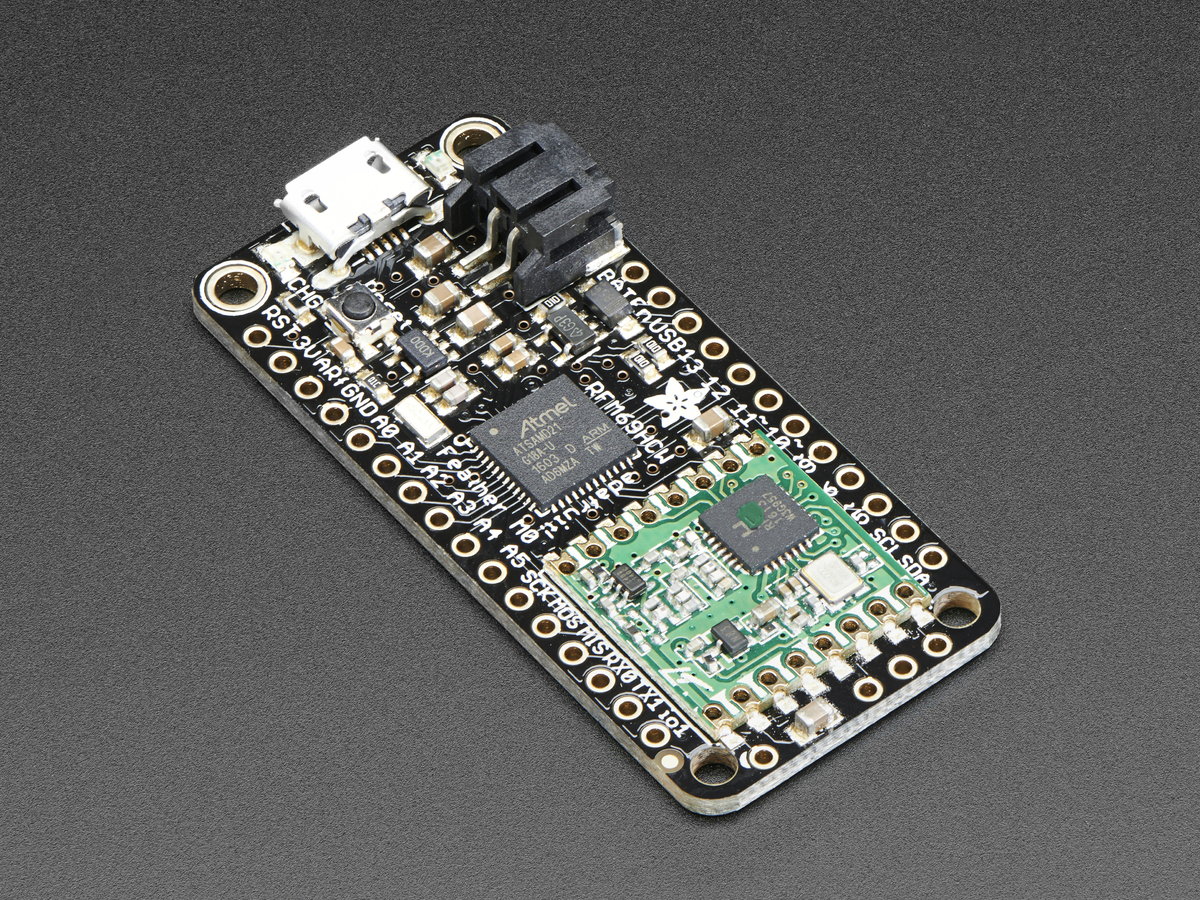
\includegraphics[width=\imgwidth]{feather.jpg}
\caption{An Adafruit Feather M0 with RFM69 Packet Radio}
\label{adafruit}
\centrefigureend

\end{enumerate}
\newpage

\section{Looking at the Spectrum}
The first thing we need to understand is what the \gls{RF} spectrum looks like. There are plenty of electromagnetic waves around, which you may or may not be aware of. Let's quickly revise what a wave looks like, by looking at \cref{wave}\footnote{\url{https://www.bbc.com/bitesize/guides/zgf97p3/revision/1}}.

\centrefigurestart
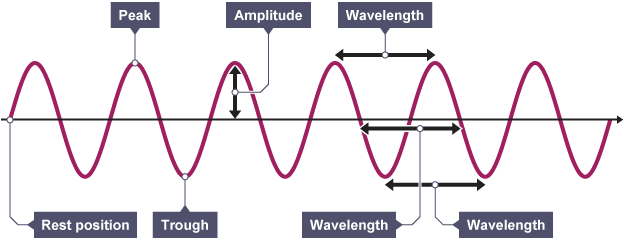
\includegraphics[width=\imgwidth]{bitesize_Wave.png}
\caption{The RF spectrum}
\label{wave}
\centrefigureend

The key thing we care about from this diagram is the wavelength because that determines how long it takes for the wave to happen; it's period. This can be used to calculate how many times it' repeats in a second, this is measured in \textit{Hertz} and is a result of the equation shown in \cref{equ:freq}. 

\begin{equation}
\text{Frequency (Hz)} = \frac{1}{\text{Time for one cycle of the wave (s)}}
\label{equ:freq}
\end{equation}

For example a signal that repeats every 2.309469 nanoseconds has a frequency of 434MHz - it repeats 434 million times a second. There are loads of different frequencies in the \gls{RF} spectrum and 434MHz fits in the \gls{uhf} part of this, as shown in \cref{spectrum}\footnote{\url{https://www.ecnmag.com/blog/2017/06/understanding-rf-spectrum}}.

\centrefigurestart
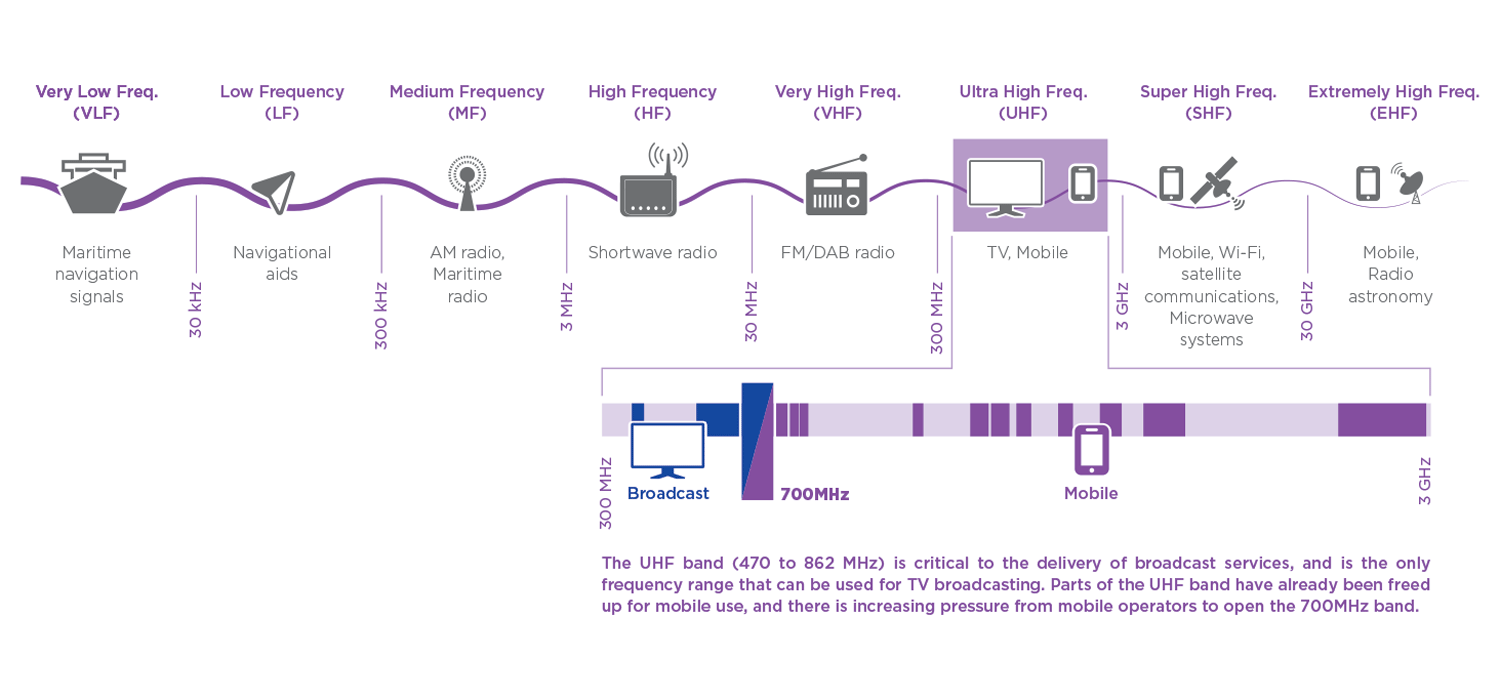
\includegraphics[width=\textwidth]{spectrum_range_services_infographic.png}
\caption{The RF spectrum}
\label{spectrum}
\centrefigureend

We can easily see the effect of these signals by using equipment which uses them; if our radio doesn't work then we know that the signals aren't present at ~90MHz. What about if we want to see a signal at 434MHz though? The radios in our car only tune into parts of the \gls{vhf} frequencies so we can't use those. Here is where our \gls{sdr} comes in useful because we can tell it a frequency to tune into (centre frequency) and we can tell it how quickly to process data (sample rate). We can then plug this into the gnuradio software to see on a graph which frequencies are most powerful, as seen in \cref{uhd_fft}.

\centrefigurestart
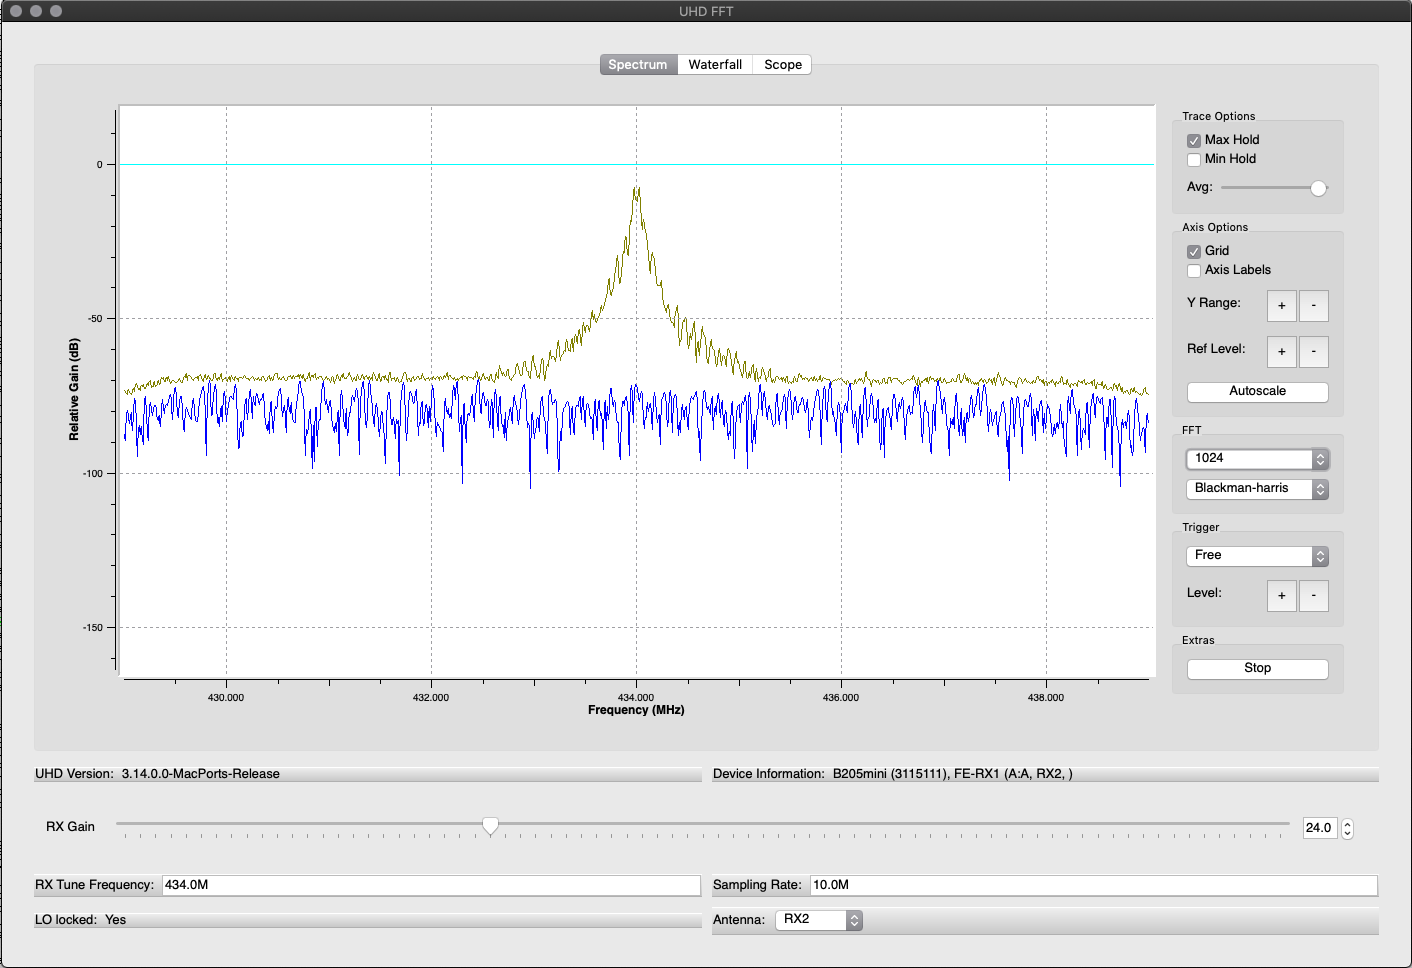
\includegraphics[width=\textwidth]{uhd_fft.png}
\caption{The output of the uhd\_fft command with a 434MHz signal present.}
\label{uhd_fft}
\centrefigureend

The spike on the yellow line in \cref{uhd_fft} shows that there is some signal present at the 434MHz frequency. We can change the settings on this window to see other signals which might be present, but first you need to run the following command from the command line to open the window.
\begin{lstlisting}
uhd_fft -f 434000000 -s 10000000
\end{lstlisting}
Try looking somewhere around 2.4GHz and seeing how busy it is. What do you think these signal might be?

\subsection{gnuradio flows}
Rather than using a prepackaged command like uht\_fft we can make our own \gls{gui}s using gnuradio companion. This can be a bit weird, so to start you off one has been provided. From the command line enter:
\begin{lstlisting}
gnuradio-companion 
\end{lstlisting}
From here open up the provided file FFT.grc and you can click the play button highlighted in \cref{grc_fft} and see the spectrum as we did before. At this point it's worth taking some time to familiarise yourself with gnuradio using the tutorial available here: \url{https://wiki.gnuradio.org/index.php/Guided\_Tutorial\_GRC}, that way it wont be a shock if the instruction is to 'add in the Throttle block', for example.

\centrefigurestart
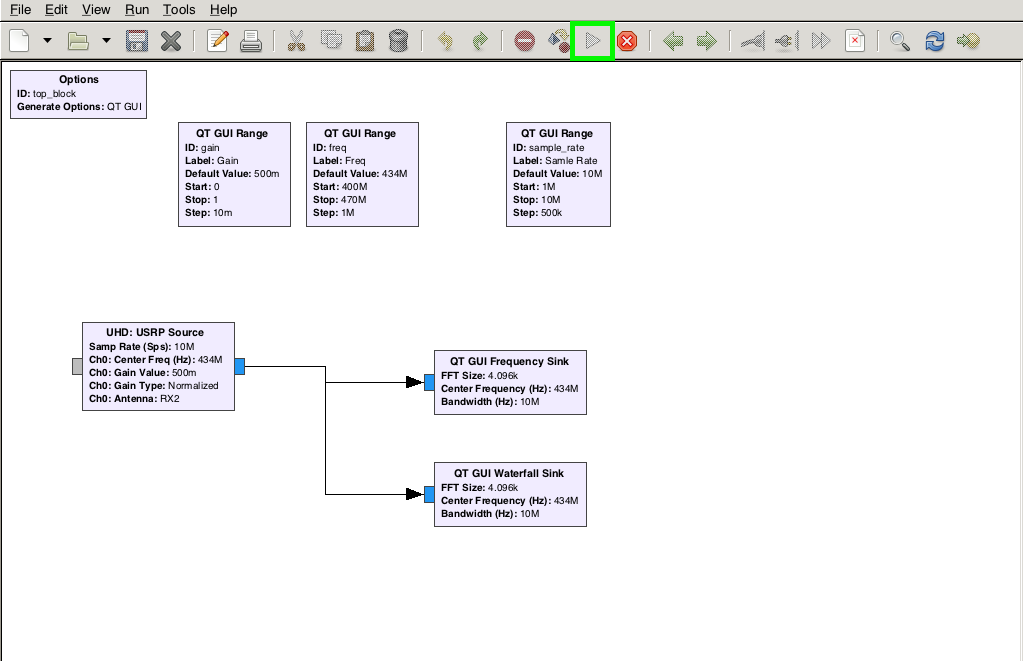
\includegraphics[width=\textwidth]{grc_fft.png}
\caption{gnuradio flow for viewing the spectrum}
\label{grc_fft}
\centrefigureend
\newpage

\section{Sending a secret message}
In this section we will use our feathers to send some messages to each other. Fortunately this is pretty simple to get started with thanks to the code provided by the RadioHead-Extras library provided.
For further information on Arduino libraries consult the Arduino website\footnote{\url{https://www.arduino.cc/en/Main/Libraries}}

\cfbox{red}{ Open up the provided SimpleFSKSend.ino sketch and the SimpleFSKRx.ino files in the Arduino editor and load them on to different feathers. } 

You should see that one is sending a message and the other is receiving it, and printing it to the serial monitor. This is our secret message! Try changing the code to send another message but for now keep the settings of the \gls{RF} chip the same, we will come back and change them later.
\newpage

\section{Spying on a secret message}
In this section we will make a custom gnuradio flow to perform a \gls{mitm} attack on our two feathers, as shown in \cref{mitm}.

\centrefigurestart
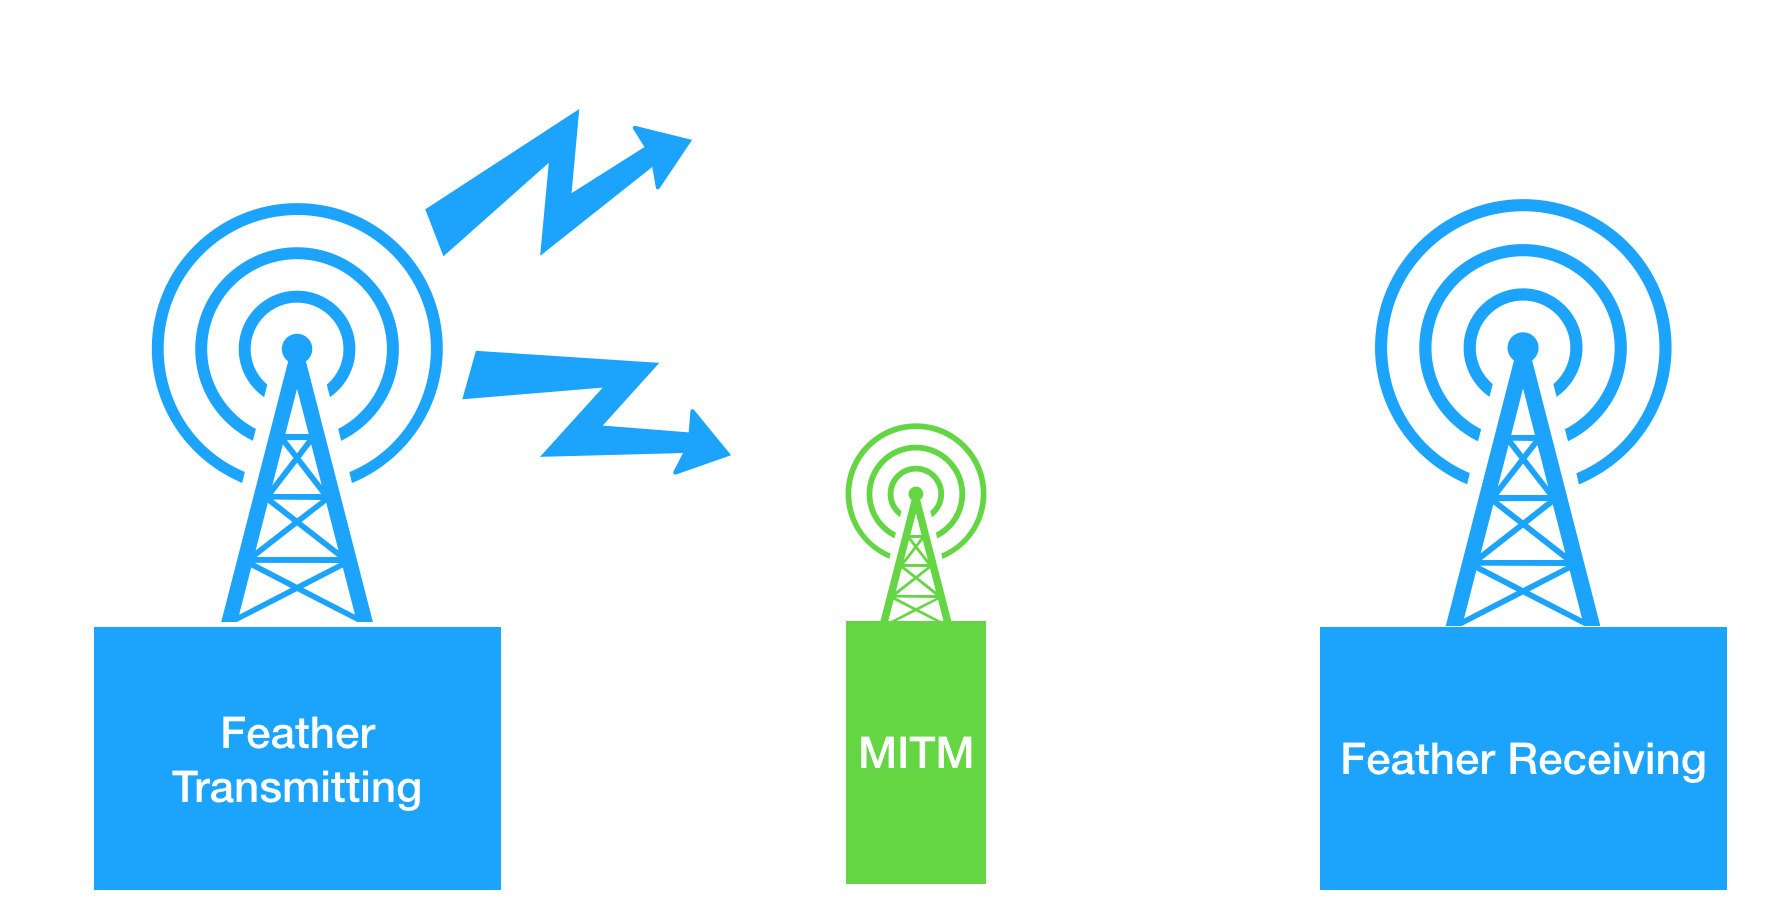
\includegraphics[width=\textwidth]{mitm.png}
\caption{MITM attack on our two feathers}
\label{mitm}
\centrefigureend

In this section will will walk through the steps to looking at the data send over the air.

\centrefigurestart
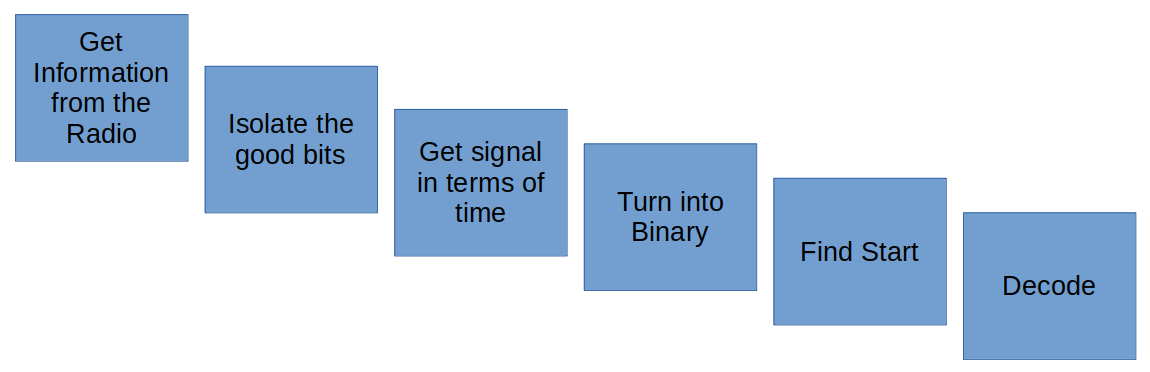
\includegraphics[width=\textwidth]{gnuflow_flow}
\caption{The steps to looking at the data sent}
\label{mitm}
\centrefigureend


\subsection{Connecting the Radio}
In order to get data into the flow from the \gls{sdr} we must use a source. In this case, it's the RTL-SDR source (In my examples I will be using a slightly different one, however the main points are the same) if there are issues there are plenty of resources available online to work through the RTL-SDR specifics \footnote{\url{https://www.instructables.com/id/RTL-SDR-FM-radio-receiver-with-GNU-Radio-Companion/}}.

Drag in the RTL-SDR source to the canvas.
\centrefigurestart
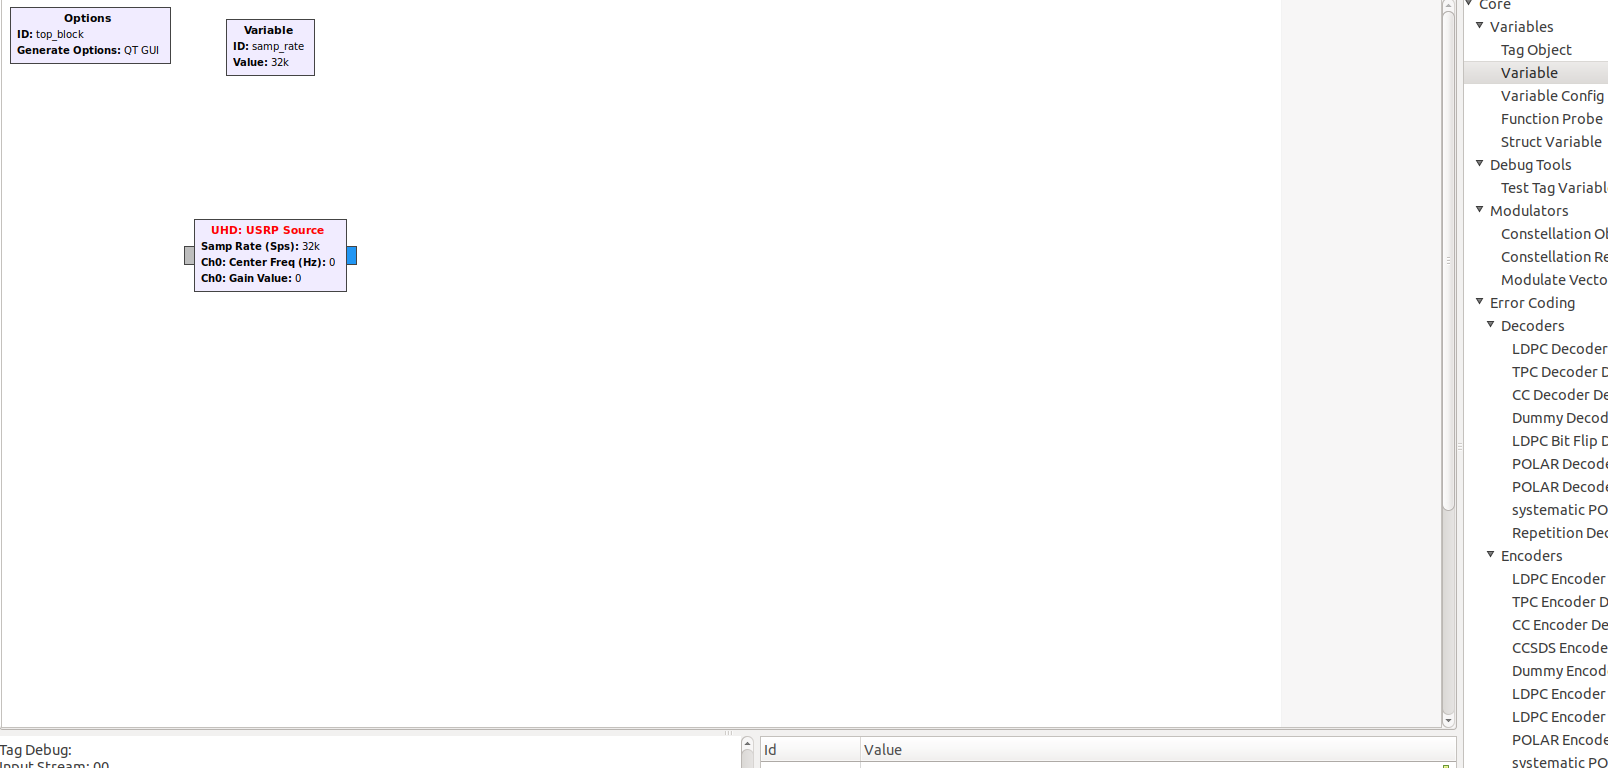
\includegraphics[width=0.5\textwidth]{rtl_src.png}
\caption{A gnuradio flow with just a radio source}
\centrefigureend

If you double click the block you will get some options, in here the key things to find are the \textit{sample rate}, \textit{gain}, and \textit{centre frequency}. The sample rate affects how quickly the radio is taking measurements (the rate at which it samples!) and as a result how wide the spectrum we are monitoring is. The gain is how loud that measurement is. The centre frequency is where the middle of the spectrum we are observing sits. The best way for us to experiment with these settings is to use the \textit{QT GUI Range} widget, this widget givs us a slider on the GUI to change settings at runtime. In order to do this, first, double click the widget's block and give it a meaningful ID, something like \textit{gain\_slider}. Give it a start value of 0, a stop value of 1, and a step of 0.1.

\centrefigurestart
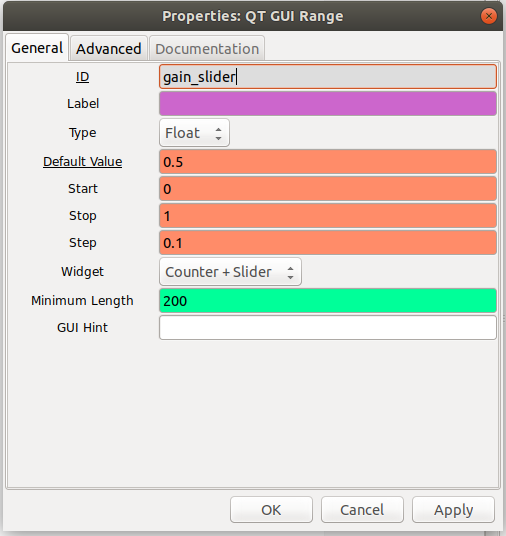
\includegraphics[width=0.5\textwidth]{range_settings}
\caption{Setting up a slider}
\centrefigureend

Now you can enter it's unique ID in the radio's settings under \textit{gain}. This is effectively telling the radio to get it's gain value from the slider called \textit{gain\_slider}.

\centrefigurestart
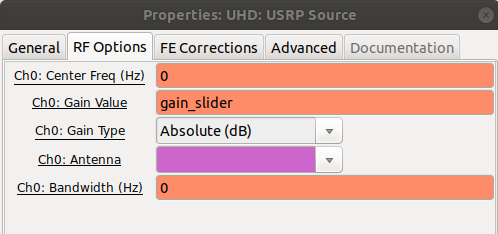
\includegraphics[width=0.5\textwidth]{gain_slider_in_usrp}
\caption{Using a slider value for the gain in the radio source.}
\centrefigureend

Do the same, creating a slider for the \textit{centre frequency} and \textit{sample rate} with the following settings:

\begin{table}[H]
\begin{tabular}{ccccc}
\hline
Setting & Start & Stop & Default & Step \\ \hline
\multicolumn{1}{|c|}{Centre Frequency} & \multicolumn{1}{c|}{430000000} & \multicolumn{1}{c|}{440000000} & \multicolumn{1}{c|}{435000000} & \multicolumn{1}{c|}{500000} \\ \hline
Sample Rate & 1000000 & 10000000 & 2000000 & 500000 \\ \hline
\end{tabular}
\caption{Radio slider settings}
\end{table}

\subsubsection{Viewing the spectrum}
The next thing is to actually be able to see the spectrum! For this a \textit{QT GUI Frequency Sink} is required. Drag this in and connect it to the radio by clicking the blue tabs.

\centrefigurestart
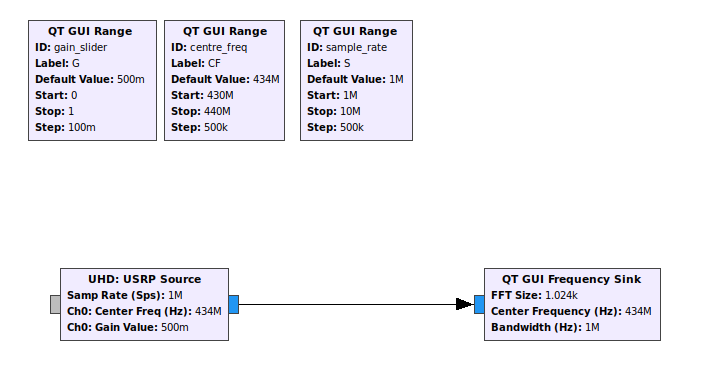
\includegraphics[width=0.5\textwidth]{basic}
\caption{A basic flow.}
\centrefigureend

Again, open the frequecy sink block and set the centre frequency to the same slider as your radio. Set the bandwidth to your sample rate slider:

\centrefigurestart
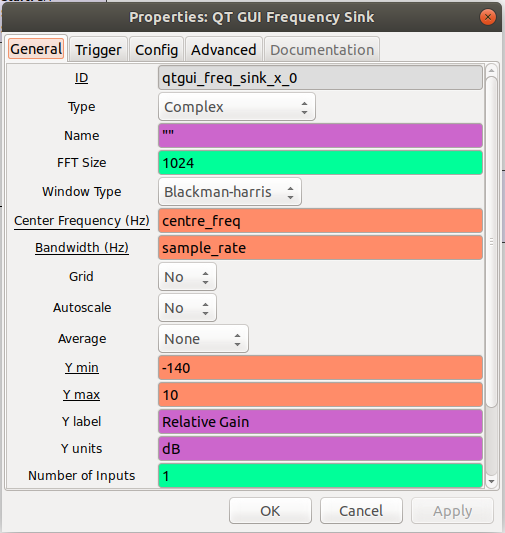
\includegraphics[width=0.5\textwidth]{fft_sink}
\caption{FFT Sink Configuration.}
\centrefigureend

While you're there, go to the \textit{Config} tab and select \textit{yes} to control panel. Now run your flow by clicking the play button at the top of the gnuradio window. This will turn your flow into a python script and run it. If there are errors address these before continuing. All being well, the window that pop up should have three sliders, and a very familiar looking spectrum. Take some time to play with the sliders and see what they do to the spectrum view. (It helps if you enable \textit{max hold} in the spectrum control panel. 

\subsection{Isolating the good bits}

The next step is to use an \gls{lpf} to make sure we receive only the transmission we are interested in. Drag an \gls{lpf} into the gnuradio flow, and add another QT Frequency Sink to see the output. In addition, it's a good idea to add some more QT Range Widgets so you can change the parameters of the filter as it's running. The parameters of interest here are the \textit{cutoff frequency} (how wide the filter is) and the \textit{transition width} (how slopey it's edges are). 

\centrefigurestart
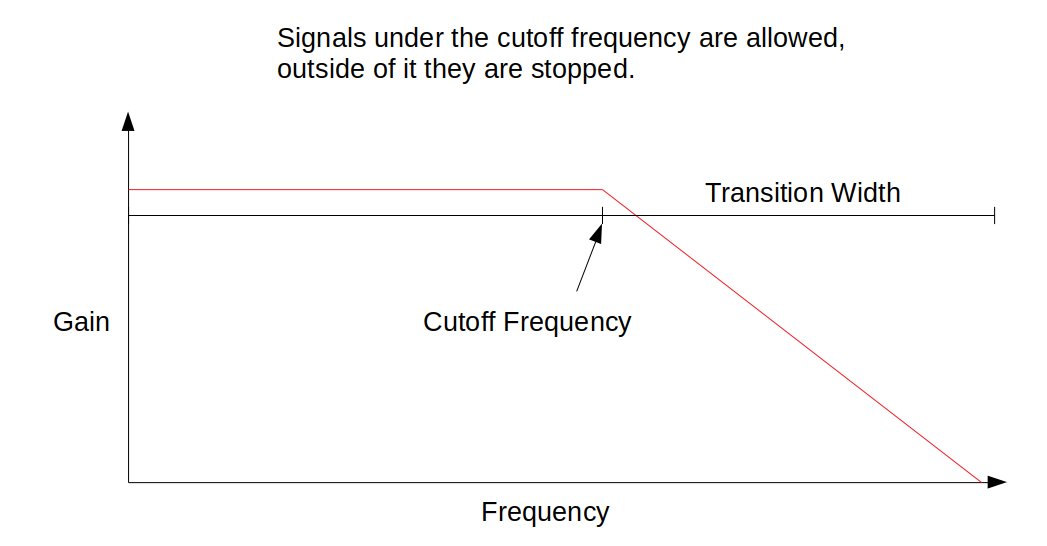
\includegraphics[width=0.5\textwidth]{lpf_filter}
\caption{Where the cutoff frequency and transition width matter.}
\centrefigureend

Our aim for the \gls{lpf} is to have an output that looks abit like barad-dur.

\begin{figure}[H]
    \centering
    \begin{minipage}{0.45\textwidth}
        \centering
        
\includegraphics[width=\textwidth]{barad_dur.jpg} 
        \caption{Sauron's home.}
    \end{minipage}\hfill
    \begin{minipage}{0.45\textwidth}
        \centering
        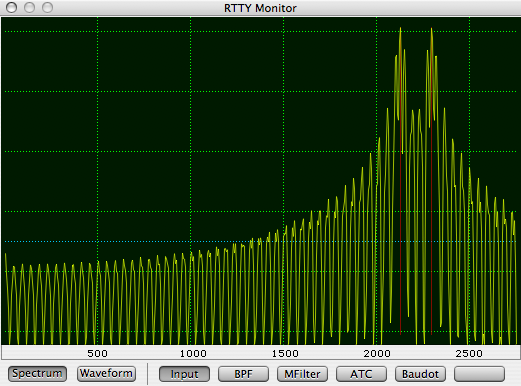
\includegraphics[width=\textwidth]{fsk_plot.png}
        \caption{FSK Signal as seen on a frequency plot.}
    \end{minipage}
\end{figure}

Run your new flow and you should be able to use the filter sliders to isolate specific parts of your signal. I found a value of around 20000 for both to give pretty good results during experimenation. We can further help our filter by using \textit{squelch}. This block will only let signals above a certain amplitude through, effectively cutting out all the noise. Put this block after your filter, and set it's \textit{alpha} to 1. Again, make a slider for it's squelch value and play with it - experiments proved that a value of -40 gave good results for me.

\centrefigurestart
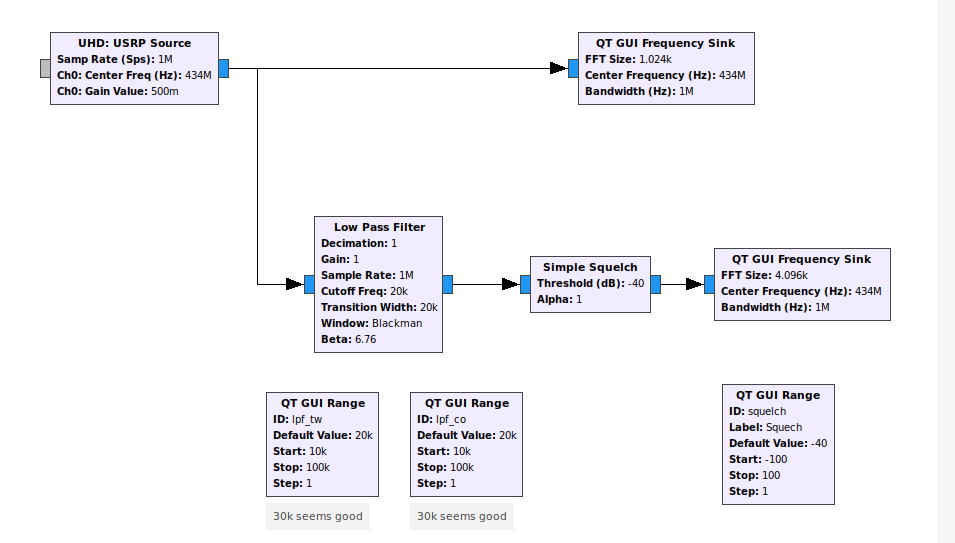
\includegraphics[width=0.5\textwidth]{squelch}
\caption{Radio - LPF - Squelch - Frequency Sink}
\centrefigureend

\subsection{Get signal in terms of time}
Now we have isolated the peaks, we can turn these into bits by using a \textit{Quadradure Demod} block with a gain setting of 1. Plug the output from this into a \textit{QT GUI Time Sink}, and enable the time sink's control panel the saem way you did with the frequency sink. 

\centrefigurestart
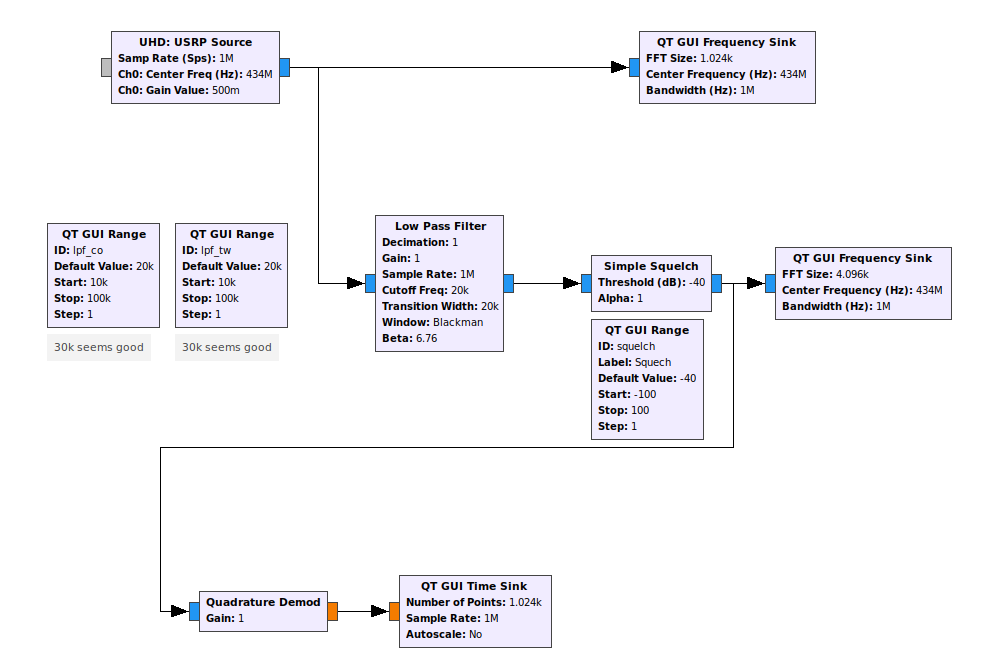
\includegraphics[width=\textwidth]{dq_flow}
\caption{Radio - LPF - Squelch - Quad Demod - Time Sink}
\centrefigureend

This new graph will have turned the frequency changes into changes against time. This will be easyier to see in the Time Sink if you set the trigger to auto, and then click '+ X Max' loads until you can see what looks like something interesting.

\centrefigurestart
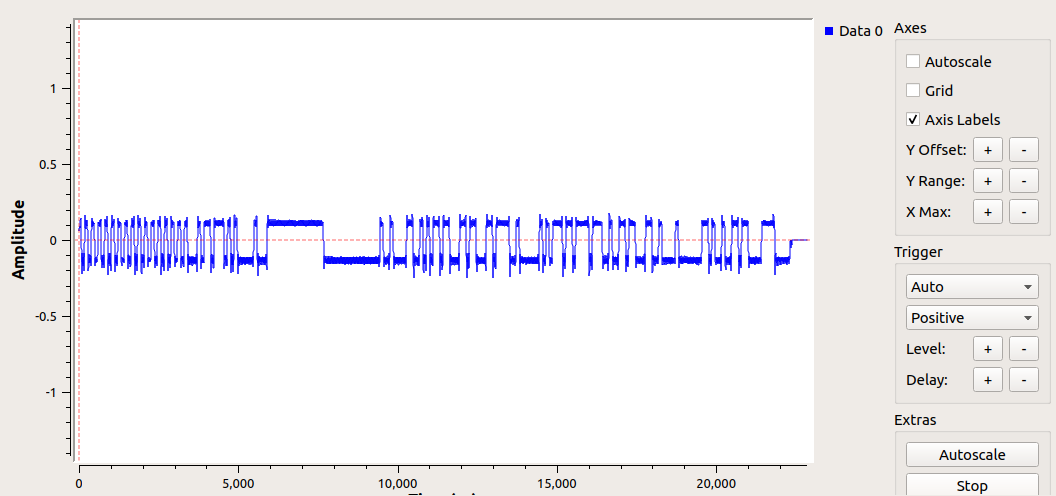
\includegraphics[width=\textwidth]{qd_time}
\caption{Our signal against time}
\centrefigureend

\subsection{Turn into binary}

In order to turn the signal into binary we need to know exactly when the transition happens. In this section we will do that using the \textit{Clock Recovery MM} block and a \textit{binary slicer}. The clock recovery relies on knowing the deviation (how far apart your peaks are in the frequency plot) and your baud rate (how quickly bits are sent in the data). Since we made the feathers talk to each other, we know these settings - so it becomes a reltively easy task of plopping numbers into an equation. In the real world however the process of finding this information may take some time and extra snooping around the RF spectrum and settings. Drag in 3 \textit{variable} blocks and use the following information:

\begin{table}[H]
\begin{tabular}{|c|c|}
\hline
\begin{tabular}[c]{@{}c@{}}Variable\\  Name\end{tabular} & Value \\ \hline
baudrate\_hz & 9600 \\ \hline
deviation\_hz & 19200 \\ \hline
\multicolumn{1}{|l|}{samples\_per\_symbol} & \multicolumn{1}{l|}{sample\_rate/baudrate\_hz} \\ \hline
\end{tabular}
\end{table}

Then, in your clock recovery block set the \textit{omega} to be \textit{samples\_per\_symbol}.

\centrefigurestart
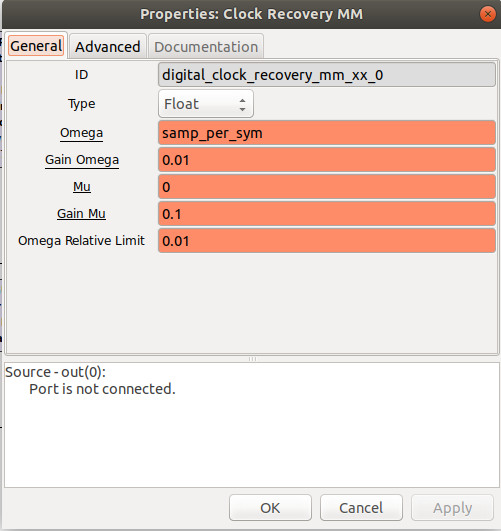
\includegraphics[width=0.5\textwidth]{clock_recovery}
\caption{Clock recovery block settings}
\centrefigureend

Again, connect a time sink to this to see the output.


\centrefigurestart
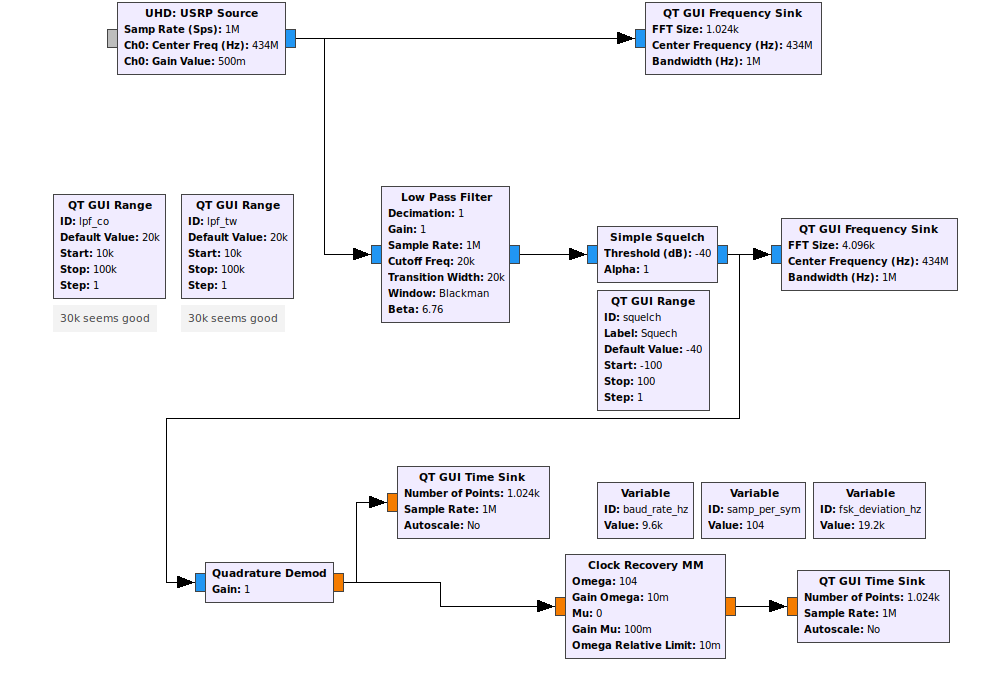
\includegraphics[width=\textwidth]{clk_recovery_flow}
\caption{Radio - Filter - Squelch - Quad Demod - Clock Recovery}
\centrefigureend

What you should see is a slight difference between the time sinks for just the quad demod and the clock recovery. The clock recovery one will look a bit pointier, and the lines will be less thick. This is clearest at the start of the graph - one data point will be high, and the next low whereas without the clock recovery this part of this signal has 'fatter' highs and lows.

\centrefigurestart
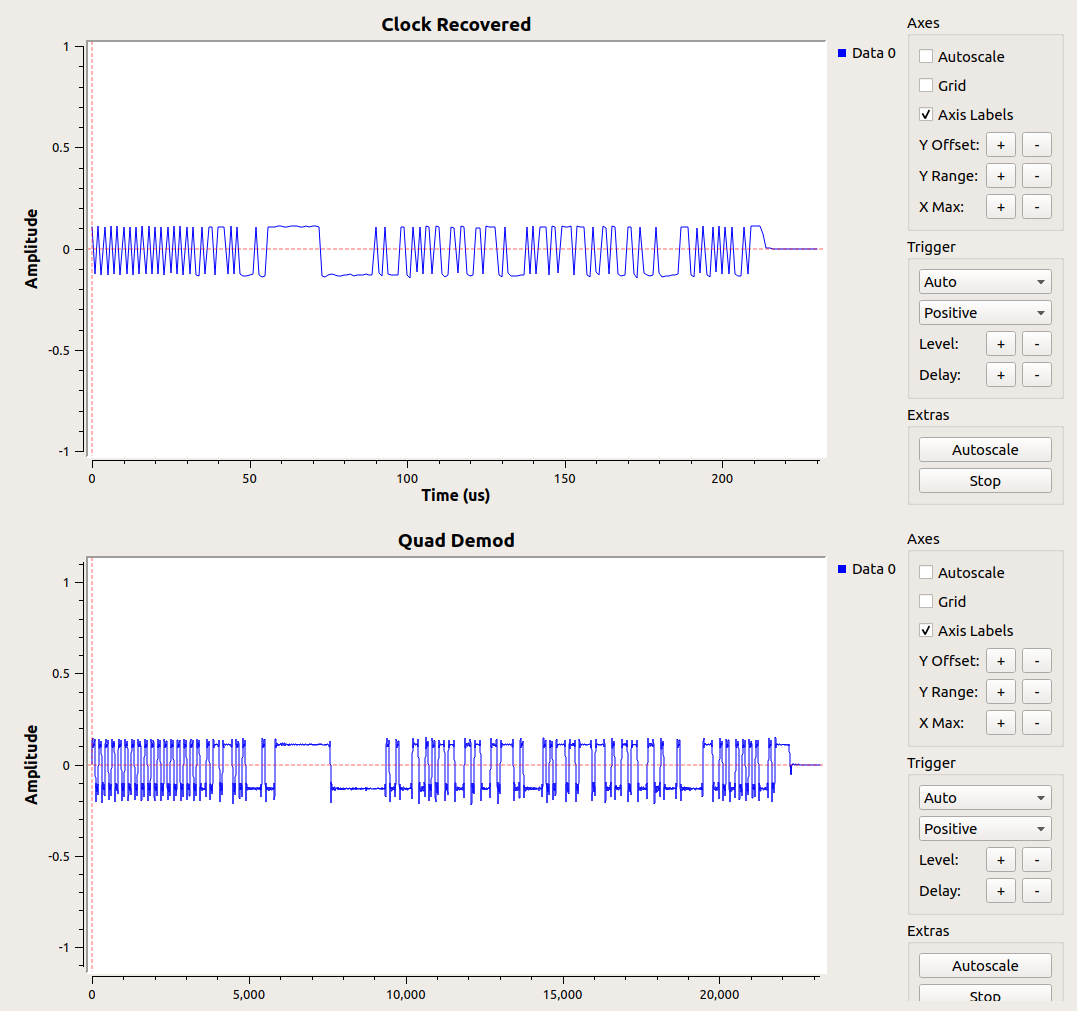
\includegraphics[width=\textwidth]{clock_vs_qd_time}
\caption{The signal before and after clock recovery}
\centrefigureend

\centrefigurestart
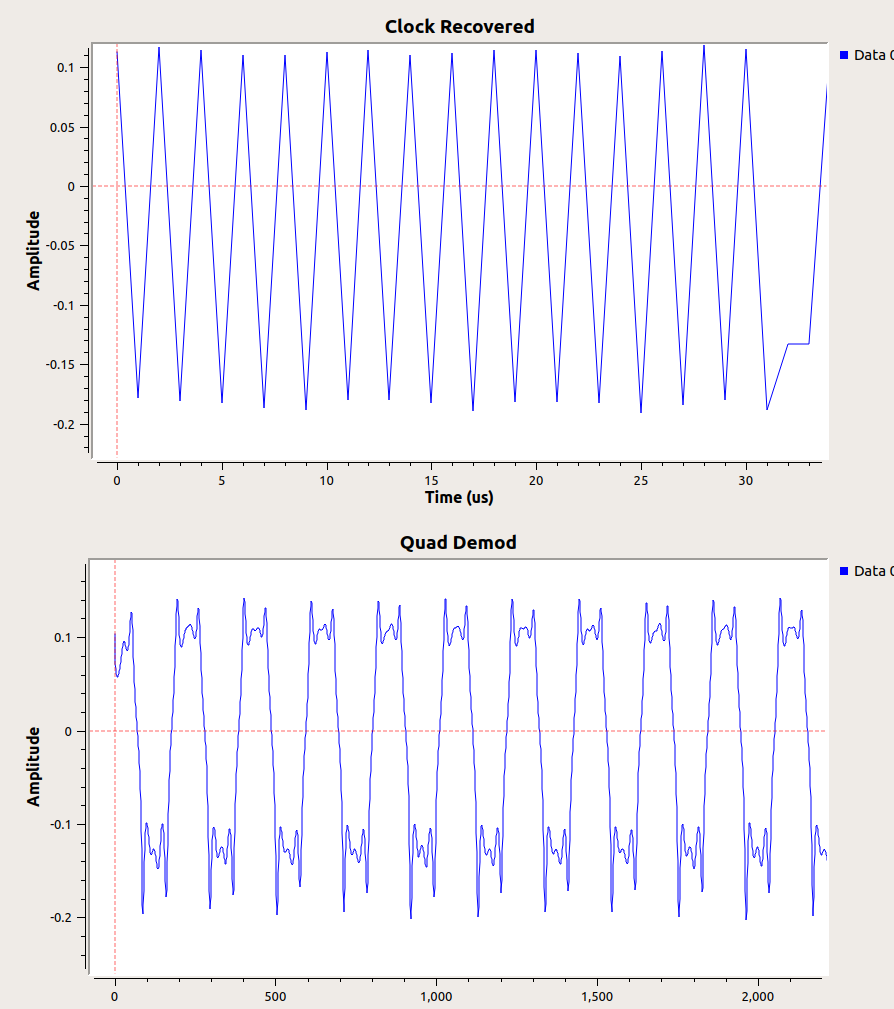
\includegraphics[width=\textwidth]{clk_recovery_vs_qd_zoom}
\caption{Detail of a series of 1 and 0 before and after clock recovery}
\centrefigureend

\subsection{Find start}

\subsection{Decode}

\newpage

\section{Real World Examples and Further Projects}
\subsection{Tyre Pressure Monitoring System}
This technique can be used in the 'real world' as demonstrated here: \url{https://www.sharebrained.com/downloads/toorcon/dude\_wheres\_my\_car\_toorcon\_sd\_2013.pdf} where someone has used the same technology to find out the tyre pressure of different cars near them. Work through the slides and the code provided and see what you can see.

\subsection{FM Reciever}
You can listen to the radio, and watch the spectrum and signals change as you do it by following the guide here: \url{https://www.instructables.com/id/RTL-SDR-FM-radio-receiver-with-GNU-Radio-Companion/}

\subsection{Satellite Images}
There is a rough guide for receiving images from weather satellites available which may require some special configuration of antenna, if you're up for it! 

\url{http://oz9aec.net/radios/gnu-radio/noaa-weather-satellite-reception-with-gnu-radio-and-usrp/}

\newpage

\end{document}
